\documentclass[10pt]{article}
\usepackage[utf8]{inputenc}
\usepackage[T1]{fontenc}
\usepackage{amsmath}
\usepackage{amsfonts}
\usepackage{amssymb}
\usepackage[version=4]{mhchem}
\usepackage{stmaryrd}
\usepackage{graphicx}
\usepackage[export]{adjustbox}
\graphicspath{ {./images/} }

\def\AA{\mathring{\mathrm{A}}}

\begin{document}
\section*{CHEMISTRY}
\section*{SECTION-A}
\begin{enumerate}
  \setcounter{enumi}{30}
  \item Given below are two statements:
\end{enumerate}

Statement I : The decrease in first ionization enthalpy from B to Al is much larger than that from Al to Ga .\\
Statement II: The d orbitals in Ga are completely filled.\\
In the light of the above statements, choose the most appropriate answer from the options given below\\
(1) Statement I is incorrect but statement II is correct.\\
(2) Both the statements I and II are correct\\
(3) Statement I is correct but statement II is incorrect\\
(4) Both the statements I and II are incorrect

Official Ans. by NTA (2)\\
Allen Ans. (1)\\
Sol. The first ionization energies (as in NCERT) are as follows:\\
B : \(801 \mathrm{~kJ} / \mathrm{mol}\)\\
Al : \(577 \mathrm{~kJ} / \mathrm{mol}\)\\
Ga : \(579 \mathrm{~kJ} / \mathrm{mol}\)\\
Ga : \([\mathrm{Ar}] 3 \mathrm{~d}^{10} 4 \mathrm{~s}^{2} 4 \mathrm{p}^{1}\)\\
32. Correct order of spin only magnetic moment of the following complex ions is:\\
(Given At. No. Fe: 26, Co:27)\\
(1) \(\left[\mathrm{FeF}_{6}\right]^{3-}>\left[\mathrm{CoF}_{6}\right]^{3-}>\left[\mathrm{Co}\left(\mathrm{C}_{2} \mathrm{O}_{4}\right)_{3}\right]^{3-}\)\\
(2) \(\left[\mathrm{Co}\left(\mathrm{C}_{2} \mathrm{O}_{4}\right)_{3}\right]^{3-}>\left[\mathrm{CoF}_{6}\right]^{3-}>\left[\mathrm{FeF}_{6}\right]^{3-}\)\\
(3) \(\left[\mathrm{FeF}_{6}\right]^{3-}>\left[\mathrm{Co}\left(\mathrm{C}_{2} \mathrm{O}_{4}\right)_{3}\right]^{3-}>\left[\mathrm{CoF}_{6}\right]^{3-}\)\\
(4) \(\left[\mathrm{CoF}_{6}\right]^{3-}>\left[\mathrm{FeF}_{6}\right]^{3-}>\left[\mathrm{Co}\left(\mathrm{C}_{2} \mathrm{O}_{4}\right)_{3}\right]^{3-}\)

Official Ans. by NTA (1)\\
Allen Ans. (1)\\
Sol. \(\left[\mathrm{FeF}_{6}\right]^{3-}: \mathrm{Fe}^{3+}=3 \mathrm{~d}^{5} \Delta_{\mathrm{O}}<\mathrm{P}\)\\
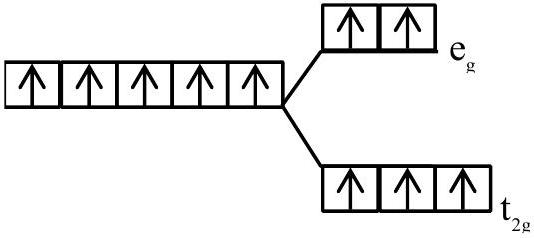
\includegraphics[max width=\textwidth, center]{2025_10_03_14e3098fda6723a79c8ag-1}

Number of unpaired \(\mathrm{e}^{-}=5 \therefore \mu=\sqrt{35} \mathrm{BM}\)

\section*{TEST PAPER WITH SOLUTION}
\(\left[\mathrm{CoF}_{6}\right]^{3-}: \mathrm{Co}^{3+}=3 \mathrm{~d}^{6}\left(\Delta_{\mathrm{O}}<\mathrm{P}\right)\)\\
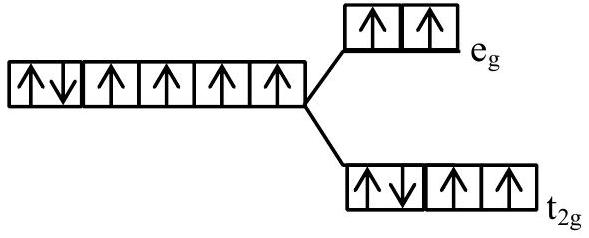
\includegraphics[max width=\textwidth, center]{2025_10_03_14e3098fda6723a79c8ag-1(1)}

Number of unpaired \(\mathrm{e}^{-}=4 \therefore \mu=\sqrt{24}\) BM\\
\(\left[\mathrm{Co}\left(\mathrm{C}_{2} \mathrm{O}_{4}\right)_{3}\right]^{3-}: \mathrm{Co}^{3+}=3 \mathrm{~d}^{6}\left(\Delta_{\mathrm{O}}>\mathrm{P}\right)\)\\
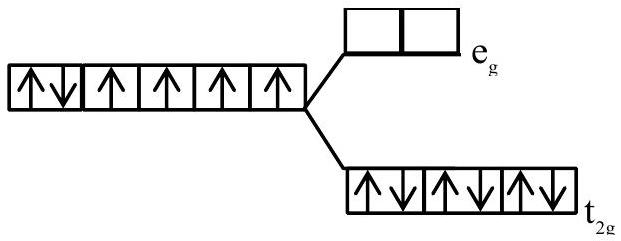
\includegraphics[max width=\textwidth, center]{2025_10_03_14e3098fda6723a79c8ag-1(2)}

Number of unpaired \(\mathrm{e}^{-}=0 \therefore \mu=0 \mathrm{BM}\)\\
33. Match List-I and List-II.

\begin{center}
\begin{tabular}{|l|l|}
\hline
List-I & List-II \\
\hline
A. Osmosis & I. Solvent molecules pass through semi permeable membrane towards solvent side. \\
\hline
B. Reverse osmosis & II. Movement of charged colloidal particles under the influence of applied electric potential towards oppositely charged electrodes. \\
\hline
C. Electro osmosis & III. Solvent molecules pass through semi permeable membrane towards solution side. \\
\hline
D. Electrophoresis & IV. Dispersion medium moves in an electric field. \\
\hline
\end{tabular}
\end{center}

Choose the correct answer from the options given below:\\
(1) A-I, B-III, C-IV, D-II\\
(2) A-III, B-I, C-IV, D-II\\
(3) A-III, B-I, C-II, D-IV\\
(4) A-I, B-III, C-II, D-IV

Official Ans. by NTA (2)\\
Allen Ans. (2)\\
Sol. A. Osmosis III\\
B. Reverse osmosis I\\
C. Electro osmosis IV\\
D. Electrophoresis II\\
34. The set of correct statements is:\\
(i) Manganese exhibits +7 oxidation state in its oxide.\\
(ii) Ruthenium and Osmium exhibit +8 oxidation in their oxides.\\
(iii) Sc shows +4 oxidation state which is oxidizing in nature.\\
(iv) Cr shows oxidising nature in +6 oxidation state.\\
(1) (ii) and (iii)\\
(2) (i), (ii) and (iv)\\
(3) (i) and (iii)\\
(4) (ii), (iii) and (iv)

Official Ans. by NTA (2)\\
Allen Ans. (2)\\
Sol. (i), (ii) and (iv) correct.\\
Manganese exhibits +7 oxidation state in its oxide. ( \(\mathrm{Mn}_{2} \mathrm{O}_{7}\) )\\
\(\mathrm{Ru} \& \mathrm{Os}\) from \(\mathrm{RuO}_{4} \& \mathrm{OsO}_{4}\) oxide in +8 oxidation state\\
Cr in +6 oxidation act is oxidizing.\\
Sc does not show +4 oxidation state.\\
35. Match List-I and List-II.

\begin{center}
\begin{tabular}{|l|l|}
\hline
List-I & List-II \\
\hline
A. Elastomeric polymer & I. Urea formaldehyde resin \\
\hline
B. Fibre polymer & II. Polystyrene \\
\hline
C. Thermosetting polymer & III. Polyester \\
\hline
D. Thermoplastic polymer & IV. Neoprene \\
\hline
\end{tabular}
\end{center}

Choose the correct answer from the options given below:\\
(1) A-II, B-III, C-I, D-IV\\
(2) A-II, B-I, C-IV, D-III\\
(3) A-IV, B-III, C-I, D-II\\
(4) A-IV, B-I, C-III, D-II

Official Ans. by NTA (3)\\
Allen Ans. (3)\\
Sol. Neoprene : Elastomer\\
Polyester : Fibre\\
Polystyrene : Thermoplastic\\
Urea-Formaldhyde Resin: Thermosetting polymer\\
36. An indicator ' \(X\) ' is used for studying the effect of variation in concentration of iodide on the rate of reaction of iodide ion with \(\mathrm{H}_{2} \mathrm{O}_{2}\) at room temp. The indicator ' X ' forms blue colored complex with compound 'A' present in the solution. The indicator ' X ' and compound ' A ' respectively are\\
(1) Starch and iodine\\
(2) Methyl orange and \(\mathrm{H}_{2} \mathrm{O}_{2}\)\\
(3) Starch and \(\mathrm{H}_{2} \mathrm{O}_{2}\)\\
(4) Methyl orange and iodine

Official Ans. by NTA (1)\\
Allen Ans. (1)\\
Sol. \(\mathrm{I}^{-}+\mathrm{H}_{2} \mathrm{O}_{2} \longrightarrow \mathrm{I}_{2}+\mathrm{H}_{2} \mathrm{O}\)\\
(A)\\
\(\mathrm{I}_{2}+\underset{\text { (Indicator) }}{\text { Starch }} \longrightarrow\) Blue\\
37. A doctor prescribed the drug Equanil to a patient. The patient was likely to have symptoms of which disease?\\
(1) Stomach ulcers\\
(2) Hyperacidity\\
(3) Anxiety and stress\\
(4) Depression and hypertension

Official Ans. by NTA (4 )\\
Allen Ans. (4)\\
Sol. Theory based.\\
38. Find out the major product for the following reaction.\\
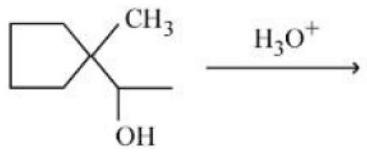
\includegraphics[max width=\textwidth, center]{2025_10_03_14e3098fda6723a79c8ag-2(1)}

Major Product\\
(1)\\
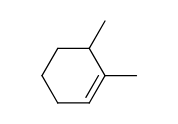
\includegraphics{smile-c2a412fd58950b128156397bef4ca7acc1afb52f}\\
(2)\\
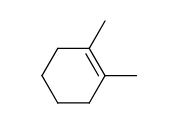
\includegraphics{smile-5e3d4f9abd7021b74eeaac6f429cb0425d48e502}\\
(3)\\
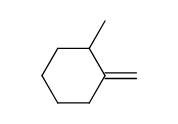
\includegraphics{smile-5bd24081a2402285606228620327e28b25506094}\\
(4)\\
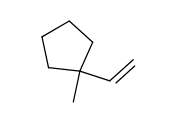
\includegraphics{smile-069aac64524912ea321917ca6531a33cdf94dab4}

Official Ans. by NTA (2)\\
Allen Ans. (2)

Sol.\\
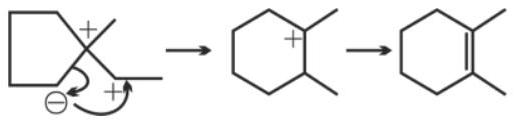
\includegraphics[max width=\textwidth, center]{2025_10_03_14e3098fda6723a79c8ag-2}\\
39. The one giving maximum number of isomeric alkenes on dehydrohalogenation reaction is (excluding rearrangement)\\
(1) 1-Bromo-2-methylbutane\\
(2) 2-Bromopropane\\
(3) 2-Bromopentane\\
(4) 2-Bromo-3,3-dimethylpentane

\section*{Official Ans. by NTA (3)}
Allen Ans. (3)

Sol.\\
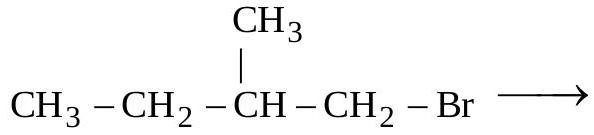
\includegraphics[max width=\textwidth, center]{2025_10_03_14e3098fda6723a79c8ag-3(1)}\\
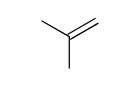
\includegraphics{smile-06162452e056e5cea8767d691bddf473b7834499}\\
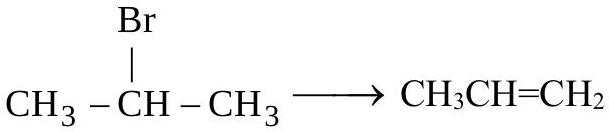
\includegraphics[max width=\textwidth, center]{2025_10_03_14e3098fda6723a79c8ag-3(3)}\\
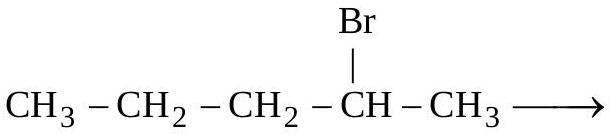
\includegraphics[max width=\textwidth, center]{2025_10_03_14e3098fda6723a79c8ag-3(2)}

\[
\mathrm{C}-\mathrm{C}-\mathrm{C}-\mathrm{C}=\mathrm{C}+\mathrm{C}-\mathrm{C}-\mathrm{C}=\mathrm{C}-\mathrm{C} \text {, cis \& trans }
\]

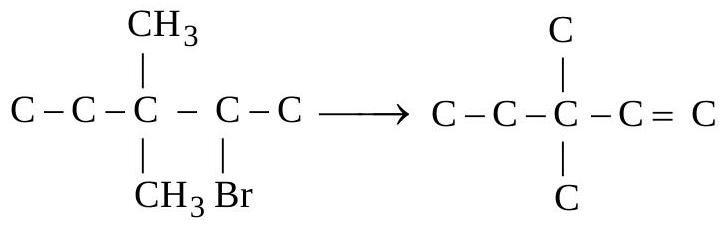
\includegraphics[max width=\textwidth, center]{2025_10_03_14e3098fda6723a79c8ag-3(4)}\\
40. When a hydrocarbon A undergoes combustion in the presence of air, it requires 9.5 equivalents of oxygen and produces 3 equivalents of water. What is the molecular formula of A ?\\
(1) \(\mathrm{C}_{8} \mathrm{H}_{6}\)\\
(2) \(\mathrm{C}_{9} \mathrm{H}_{9}\)\\
(3) \(\mathrm{C}_{6} \mathrm{H}_{6}\)\\
(4) \(\mathrm{C}_{9} \mathrm{H}_{6}\)

Official Ans. by NTA (1)\\
Allen Ans. (1)\\
Sol. \(\quad \mathrm{C}_{\mathrm{x}} \mathrm{H}_{\mathrm{y}}+\left(\mathrm{x}+\frac{\mathrm{y}}{4}\right) \mathrm{O}_{2} \rightarrow \mathrm{xCO}_{2}+\frac{\mathrm{y}}{2} \mathrm{H}_{2} \mathrm{O}\)\\
\(\mathrm{x}+\frac{\mathrm{y}}{4}=9.5\)\\
\(\frac{\mathrm{y}}{2}=3\)\\
\(\Rightarrow \mathrm{x}=8, \mathrm{y}=6\)\\
41. Find out the major products from the following reaction sequence.\\
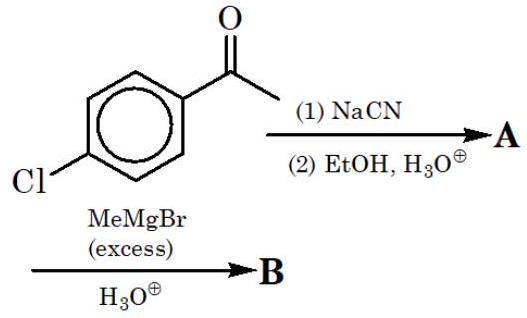
\includegraphics[max width=\textwidth, center]{2025_10_03_14e3098fda6723a79c8ag-3}\\
(1)\\
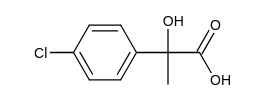
\includegraphics{smile-94e3b3092ec3d071e1554b2598290be3bc581073}\\
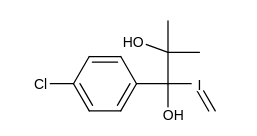
\includegraphics{smile-ba3d8c81b4d70e34ba71924f339723275cbf5ecd}\\
(2)\\
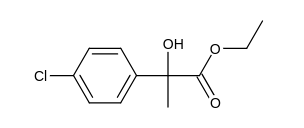
\includegraphics{smile-14f70836d113413a93496c3908b18ac0cb261aab}\\
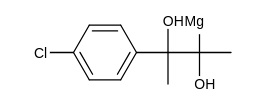
\includegraphics{smile-dcde5cba7d57816b31f54c26a7f71ba0a8903242}\\
(3)\\
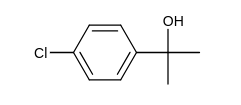
\includegraphics{smile-628ac770507c43d501bc89784fcd3bd997f109d3}\\
(4)\\
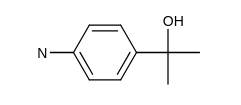
\includegraphics{smile-41280cd0991fafbb5aa2bd449f1e05acdfa932a1}\\
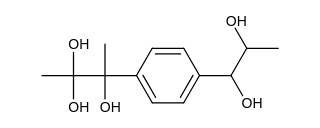
\includegraphics{smile-b25ec32f25149bb0d7bd95a0ca7b6cb596ef96f5}

Official Ans. by NTA (2 )\\
Allen Ans. (2)

Sol.\\
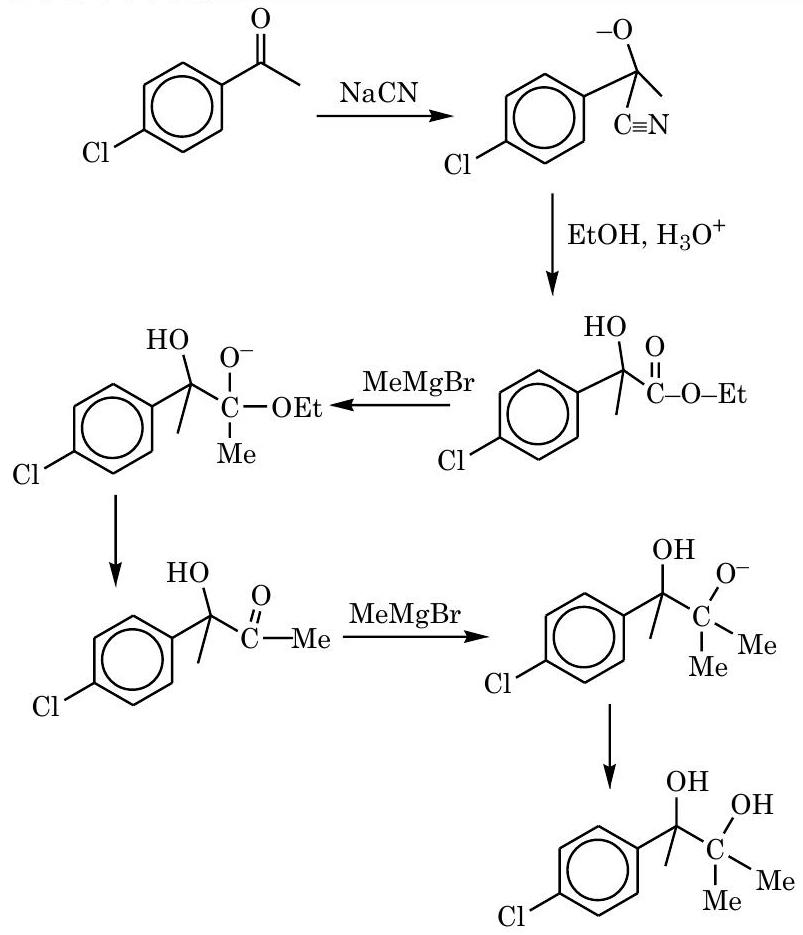
\includegraphics[max width=\textwidth, center]{2025_10_03_14e3098fda6723a79c8ag-4(1)}\\
42. According to MO theory the bond orders for \(\mathrm{O}_{2}{ }^{2-}\), CO and \(\mathrm{NO}^{+}\)respectively, are\\
(1) 1, 3 and 3\\
(2) 1, 3 and 2\\
(3) 1, 2 and 3\\
(4) 2, 3 and 3

Official Ans. by NTA (1)\\
Allen Ans. (1)\\
Sol. Theory based.\\
43. A solution of \(\mathrm{CrO}_{5}\) in amyl alcohol has a....colour\\
(1) Green\\
(2) Orange-Red\\
(3) Yellow\\
(4) Blue

Official Ans. by NTA (4)\\
Allen Ans. (4)\\
Sol. A solution of \(\mathrm{CrO}_{5}\) in amyl alcohol has a blue colour. So, option (4) is correct.\\
44. The concentration of dissolved Oxygen in water for growth of fish should be more than \(\underline{X} \mathrm{ppm}\) and Biochemical Oxygen Demand in clean water should be less than \(\underline{Y}\) ppm. \(X\) and \(Y\) in ppm are, respectively.\\
(1) \(\mathrm{X} \quad \mathrm{Y}\)\\
(2) \(\begin{array}{ll}X & Y \\ 4 & \end{array}\)\\
65\\
48\\
(3) X Y\\
(4) X Y\\
(3)\\
415\\
(4)\\
612

\section*{Official Ans. by NTA (1)}
Allen Ans. (1)\\
Sol. The growth of fish gets inhibited if the concentration of dissolved Oxygen in water is less than 6 ppm and Biochemical Oxygen demand in clean water should be less than 5 ppm .

\[
\begin{gathered}
\mathrm{Ph}-\mathrm{CH}_{2}-\mathrm{CH}-\mathrm{COOH} \\
\mathrm{NH}_{2} \\
\text { (F) } \\
\text { (Phenylalanine) }
\end{gathered}
\]

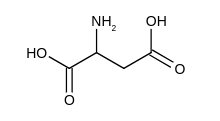
\includegraphics{smile-a5f6468b0c5c3f9889de7263f9f72008bb65fd57}\\
(D)\\
(Aspartic acid)\\
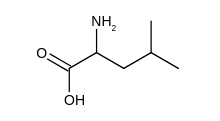
\includegraphics{smile-3e9c14c983d5a42364f0c8e873a9b1227ffdd8d8}\\
(L)\\
(Leucine)\\
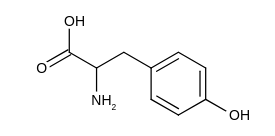
\includegraphics{smile-79314ca6ce05e9e0de07ed11408d3def65e7c769}\\
(Y)\\
(Tyrosine)\\
45. Reaction of propanamide with \(\mathrm{Br}_{2} / \mathrm{KOH}(\mathrm{aq})\) produces :\\
(1) Ethylnitrile\\
(2) Propylamine\\
(3) Propanenitrile\\
(4) Ethylamine

Official Ans. by NTA (4)\\
Allen Ans. (4)

Sol.\\
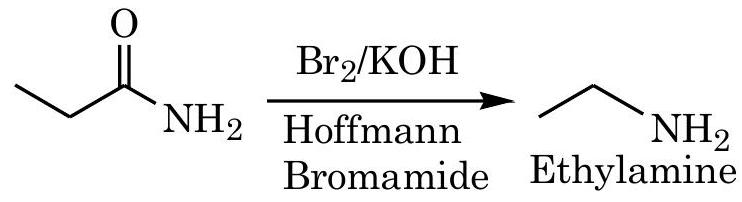
\includegraphics[max width=\textwidth, center]{2025_10_03_14e3098fda6723a79c8ag-4}\\
46. Following tetrapeptide can be represented as\\
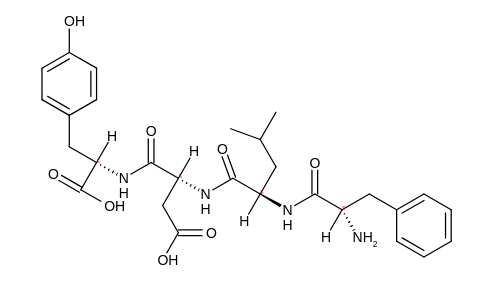
\includegraphics{smile-f85d8aaf784452892eebe5e4238f69d7736b6241}\\
( \(\mathrm{F}, \mathrm{L}, \mathrm{D}, \mathrm{Y}, \mathrm{I}, \mathrm{Q}, \mathrm{P}\) are one letter codes for amino acids)\\
(1) FIQY\\
(2) FLDY\\
(3) YQLF\\
(4) PLDY

Official Ans. by NTA (2)\\
Allen Ans. (2)\\
Sol. Hydrolysis of the given tetrapeptide will give the following:\\
47. Which of the following relations are correct?\\
(A) \(\Delta \mathrm{U}=\mathrm{q}+\mathrm{p} \Delta \mathrm{V}\)\\
(B) \(\Delta \mathrm{G}=\Delta \mathrm{H}-\mathrm{T} \Delta \mathrm{S}\)\\
(C) \(\Delta S=\frac{q_{\text {rev }}}{T}\)\\
(D) \(\Delta \mathrm{H}=\Delta \mathrm{U}-\Delta \mathrm{nRT}\)

Choose the most appropriate answer from the options given below :\\
(1) C and D only\\
(2) B and C only\\
(3) A and B only\\
(4) B and D only

\section*{Official Ans. by NTA (2)}
\section*{Allen Ans. (2)}
Sol. Only (B) and (C) are correct.\\
(B) \(\mathrm{G}=\mathrm{H}-\mathrm{TS}\)

At constant T

\[
\Delta G=\Delta H-T \Delta S
\]

(A) First law is given by

\[
\Delta U=Q+W
\]

If we apply constant P and reversible work.

\[
\Delta U=Q-P \Delta V
\]

(C)By definition of entropy change

\[
\mathrm{dS}=\frac{\mathrm{dq}_{\mathrm{rev}}}{\mathrm{~T}}
\]

At constant T

\[
\Delta \mathrm{S}=\frac{\mathrm{q}_{\mathrm{rev}}}{\mathrm{~T}}
\]

(D) \(\mathrm{H}=\mathrm{U}+\mathrm{PV}\)

For ideal gas\\
\(\mathrm{H}=\mathrm{U}+\mathrm{nRT}\)\\
At constant T\\
\(\Delta \mathrm{H}=\Delta \mathrm{U}+\Delta \mathrm{nRT}\)\\
48. The major component of which of the following ore is sulphide based mineral?\\
(1) Calamine\\
(2) Siderite\\
(3) Sphalerite\\
(4) Malachite

\section*{Official Ans. by NTA (3)}
\section*{Allen Ans. (3)}
Sol. Calamine : \(\mathrm{ZnCO}_{3}\)\\
Siderite : \(\mathrm{FeCO}_{3}\)\\
Sphalerite : ZnS\\
Malachite : \(\mathrm{CuCO}_{3} . \mathrm{Cu}(\mathrm{OH})_{2}\)\\
49. Given below are two statements:

Statement I : Nickel is being used as the catalyst for producing syn gas and edible fats.\\
Statement II : Silicon forms both electron rich and electron deficient hydrides.\\
In the light of the above statements, choose the most appropriate answer from the options given below:\\
(1) Both the statements I and II are correct\\
(2) Statement I is incorrect but statement II is correct\\
(3) Both the statements I and II are incorrect\\
(4) Statement I is correct but statement II is incorrect\\
Official Ans. by NTA (4)\\
Allen Ans. (4)\\
Sol. Statement-I is correct.\\
Ni is used in Hydrogenation of unsaturated fat to make edible fats.\\
Statements-II is false as hydride of Silicon is electron precise \& neither electron deficient nor electron rich.\\
50. Match List I with List II.

\begin{center}
\begin{tabular}{|l|l|l|l|}
\hline
\multicolumn{2}{|c|}{List I} & \multicolumn{2}{|c|}{List II} \\
\hline
A. & van't Hoff factor, i & I. & Cryoscopic constant \\
\hline
B. & \(\mathrm{k}_{\mathrm{f}}\) & II. & Isotonic solutions \\
\hline
C. & Solutions with same osmotic pressure & III. & \begin{tabular}{l}
Normal molar mass \\
Abnormal molar mass \\
\end{tabular} \\
\hline
D. & Azeotropes & IV. & Solutions with same composition of vapour above it \\
\hline
\end{tabular}
\end{center}

Choose the correct answer from the options given below :\\
(A) A-III, B-I, C-II, D-IV\\
(B) A-III, B-II, C-I, D-IV\\
(C) A-III, B-I, C-IV, D-II\\
(D) A-I, B-III, C-II, D-IV

Official Ans. by NTA (1)\\
Allen Ans. (1)\\
Sol. (A) van't Hoff factor, i

\[
\mathrm{i}=\frac{\text { Normal molar mass }}{\text { Abnormal molar mass }}
\]

(B) \(\mathrm{k}_{\mathrm{f}}=\) Cryoscopic constant\\
(C) Solutions with same osmotic pressure are known as isotonic solutions.\\
(D) Solutions with same composition of vapour over them are called Azeotrope.

\section*{SECTION-B}
\begin{enumerate}
  \setcounter{enumi}{50}
  \item On heating, \(\mathrm{LiNO}_{3}\) gives how many compounds among the following?\\
\(\mathrm{Li}_{2} \mathrm{O}, \mathrm{N}_{2}, \mathrm{O}_{2}, \mathrm{LiNO}_{2}, \mathrm{NO}_{2}\)\\
Official Ans. by NTA (3)\\
Allen Ans. (3)\\
Sol. \(2 \mathrm{Li} \mathrm{NO}_{3} \xrightarrow{\Delta} \mathrm{Li}_{2} \mathrm{O}+2 \mathrm{NO}_{2}+\frac{1}{2} \mathrm{O}_{2}\)\\
Hence three products \(\mathrm{Li}_{2} \mathrm{O}, \mathrm{NO}_{2}\) and \(\mathrm{O}_{2}\)
  \item At 298 K\\
\(\mathrm{N}_{2}(\mathrm{~g})+3 \mathrm{H}_{2}(\mathrm{~g}) \rightleftharpoons 2 \mathrm{NH}_{3}(\mathrm{~g}), \mathrm{K}_{1}=4 \times 10^{5}\)\\
\(\mathrm{N}_{2}(\mathrm{~g})+\mathrm{O}_{2}(\mathrm{~g}) \rightleftharpoons 2 \mathrm{NO}(\mathrm{g}), \mathrm{K}_{2}=1.6 \times 10^{12}\)\\
\(\mathrm{H}_{2}(\mathrm{~g})+\frac{1}{2} \mathrm{O}_{2}(\mathrm{~g}) \rightleftharpoons \mathrm{H}_{2} \mathrm{O}(\mathrm{g}), \mathrm{K}_{3}=1.0 \times 10^{-13}\)\\
Based on above equilibria, the equilibrium constant of the reaction,\\
\(2 \mathrm{NH}_{3}(\mathrm{~g})+\frac{5}{2} \mathrm{O}_{2}(\mathrm{~g}) \rightleftharpoons 2 \mathrm{NO}(\mathrm{g})+3 \mathrm{H}_{2} \mathrm{O}(\mathrm{g})\)\\
is \(\_\_\_\_\) \(\times 10^{-33}\)\\
(Nearest integer)
\end{enumerate}

\section*{Official Ans. by NTA (4)}
\section*{Allen Ans. (4)}
Sol. \(\mathrm{N}_{2}(\mathrm{~g})+3 \mathrm{H}_{2}(\mathrm{~g}) \rightleftharpoons 2 \mathrm{NH}_{3}(\mathrm{~g}), \mathrm{K}_{1}=4 \times 10^{5}\)

\[
\mathrm{N}_{2}(\mathrm{~g})+\mathrm{O}_{2}(\mathrm{~g}) \rightleftharpoons 2 \mathrm{NO}(\mathrm{~g}), \mathrm{K}_{2}=1.6 \times 10^{12}
\]

\[
\mathrm{H}_{2}(\mathrm{~g})+\frac{1}{2} \mathrm{O}_{2}(\mathrm{~g}) \rightleftharpoons \mathrm{H}_{2} \mathrm{O}(\mathrm{~g}), \mathrm{K}_{3}=1.0 \times 10^{-13}
\]

(ii) \(+3 \times\) (iii) - (i)\\
\(2 \mathrm{NH}_{3}(\mathrm{~g})+\frac{5}{2} \mathrm{O}_{2}(\mathrm{~g}) \rightleftharpoons 2 \mathrm{NO}(\mathrm{g})+3 \mathrm{H}_{2} \mathrm{O}(\mathrm{g})\)

\[
\begin{aligned}
\mathrm{k}_{\mathrm{eq}} & =\frac{\mathrm{k}_{2} \times \mathrm{k}_{3}^{3}}{\mathrm{k}_{1}}=\frac{1.6 \times 10^{12} \times\left(10^{-13}\right)^{3}}{4 \times 10^{5}} \\
& =\frac{1.6}{4} \times 10^{-32}=4 \times 10^{-33}
\end{aligned}
\]

\begin{enumerate}
  \setcounter{enumi}{52}
  \item For conversion of compound \(\mathrm{A} \rightarrow \mathrm{B}\), the rate constant of the reaction was found to be \(4.6 \times 10^{-5} \mathrm{L} \mathrm{mol}^{-1} \mathrm{~s}^{-1}\). The order of the reaction is \(\_\_\_\_\) .
\end{enumerate}

\section*{Official Ans. by NTA (2)}
\section*{Allen Ans. (2)}
Sol. As unit of rate constant is (conc.) \({ }^{1-n}\) time \(^{-1}\)

\[
\Rightarrow\left(\mathrm{L} \mathrm{~mol}^{-1}\right) \Rightarrow 1-\mathrm{n}=-1 \quad \mathrm{n}=2
\]

\begin{enumerate}
  \setcounter{enumi}{53}
  \item Total number of acidic oxides among\\
\(\mathrm{N}_{2} \mathrm{O}_{3}, \mathrm{NO}_{2}, \mathrm{~N}_{2} \mathrm{O}, \mathrm{Cl}_{2} \mathrm{O}_{7}, \mathrm{SO}_{2}, \mathrm{CO}, \mathrm{CaO}, \mathrm{Na}_{2} \mathrm{O}\) and NO is \(\_\_\_\_\) .\\
Official Ans. by NTA (4 )\\
Allen Ans. (4)\\
Sol. Acidic oxides are \(\mathrm{N}_{2} \mathrm{O}_{3}, \mathrm{NO}_{2}, \mathrm{Cl}_{2} \mathrm{O}_{7}, \mathrm{SO}_{2}\)
  \item When 0.01 mol of an organic compound containing \(60 \%\) carbon was burnt completely, 4.4 g of \(\mathrm{CO}_{2}\) was produced. The molar mass of compound is\\
\(\_\_\_\_\) g \(\mathrm{mol}^{-1}\) (Nearest integer)\\
Official Ans. by NTA (200)\\
Allen Ans. (200)\\
Sol. Let M is the molar mass of the compound ( \(\mathrm{g} / \mathrm{mol}\) )\\
mass of compound \(=0.01 \mathrm{Mgm}\)\\
mass of carbon \(=0.01 \mathrm{M} \times \frac{60}{100}\)\\
moles of carbon \(=\frac{0.01 \mathrm{M}}{12} \times \frac{60}{100}\)\\
moles of \(\mathrm{CO}_{2}\) from combustion \(=\frac{4.4}{44}=\) moles of carbon\\
\(\frac{0.01 \mathrm{M}}{12} \times \frac{60}{100}=\frac{4.4}{44}\)\\
\(M=\frac{4.4}{44} \times \frac{100}{60} \times \frac{12}{0.01}=200 \mathrm{gm} / \mathrm{mol}\)
  \item The denticity of the ligand present in the Fehling's reagent is \(\_\_\_\_\) .\\
Official Ans. by NTA (4)\\
Allen Ans. (4)\\
Sol.\\
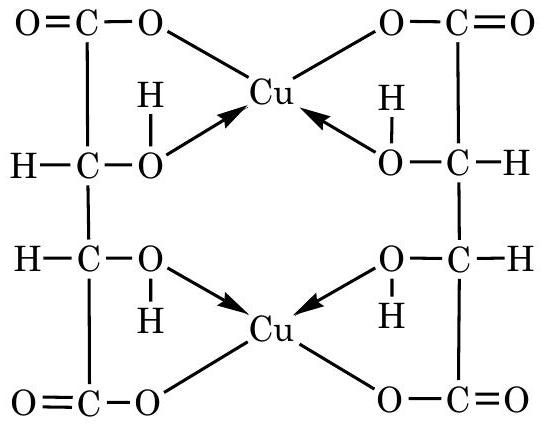
\includegraphics[max width=\textwidth, center]{2025_10_03_14e3098fda6723a79c8ag-6}
\end{enumerate}

Copper tartarate complex\\
Denticity \(=2\)\\
57. A metal M forms hexagonal close-packed structure. The total number of voids in 0.02 mol of it is \(\_\_\_\_\) \(\times 10^{21}\) (Nearest integer)\\
(Given \(\mathrm{N}_{\mathrm{A}}=6.02 \times 10^{23}\) )\\
Official Ans. by NTA (36)\\
Allen Ans. (36)

Sol. One unit cell of hcp contains \(=18\) voids\\
No. of voids in 0.02 mol of hcp\\
\(=\frac{18}{6} \times 6.02 \times 10^{23} \times 0.02\)\\
\(\approx 3.6 \times 10^{22}\)\\
\(\approx 36 \times 10^{21}\)\\
58. Assume that the radius of the first Bohr orbit of hydrogen atom is \(0.6 \AA\). The radius of the third Bohr orbit of \(\mathrm{He}^{+}\)is \(\_\_\_\_\) picometer. (Nearest Integer)

Official Ans. by NTA (270)\\
Allen Ans. (270)\\
Sol. \(r \propto \frac{n^{2}}{Z}\)\\
\(\mathrm{r}_{\mathrm{He}^{+}}=\mathrm{r}_{\mathrm{H}} \times \frac{\mathrm{n}^{2}}{\mathrm{Z}}\)\\
\(\mathrm{r}_{\mathrm{He}^{+}}=0.6 \times \frac{(3)^{2}}{2}\)\\
\(=2.7 \AA\)\\
\(\mathrm{r}_{\mathrm{He}^{+}}=270 \mathrm{pm}\)\\
59. The equilibrium constant for the reaction\\
\(\mathrm{Zn}(\mathrm{s})+\mathrm{Sn}^{2+}(\mathrm{aq}) \rightleftharpoons \mathrm{Zn}^{2+}(\mathrm{aq})+\mathrm{Sn}(\mathrm{s})\) is \(1 \times 10^{20}\) at 298 K . The magnitude of standard electrode potential of \(\mathrm{Sn} / \mathrm{Sn}^{2+}\) if \(\mathrm{E}_{\mathrm{Zn}^{2+} / \mathrm{Zn}}^{\mathrm{o}}=-0.76 \mathrm{~V}\) is\\
\(\_\_\_\_\) \(\times 10^{-2} \mathrm{~V}\). (Nearest integer)

Given : \(\frac{2.303 R T}{F}=0.059 \mathrm{~V}\)\\
Official Ans. by NTA (17)\\
Allen Ans. (17)\\
Sol. \(\mathrm{Zn}(\mathrm{s})+\mathrm{Sn}^{2+}(\mathrm{aq}) \rightleftharpoons \mathrm{Zn}^{2+}(\mathrm{aq})+\mathrm{Sn}(\mathrm{s})\)\\
\(\Delta \mathrm{G}^{\circ}=-2.303 \mathrm{RT} \log _{10} \mathrm{Keq}\)\\
\(-n F\left(E_{\text {cell }}^{0}\right)=-2.303 R T \log _{10}\) Keq\\
\(\mathrm{E}_{\mathrm{Zn} / \mathrm{Zn}^{2+}}^{0}+\mathrm{E}_{\mathrm{Sn}^{2+} / \mathrm{Sn}}^{0}=\frac{0.059}{2} \log _{10} \mathrm{Keq}\)\\
\(0.76+\mathrm{E}_{\mathrm{Sn}^{2+} / \mathrm{Sn}}^{0}=\frac{0.059}{2} \log _{10} 10^{20}\)\\
\(0.76+\mathrm{E}_{\mathrm{Sn}^{2+} / \mathrm{Sn}}^{0}=\frac{0.059 \times 20}{2}\)\\
\(\mathrm{E}_{\mathrm{Sn}^{2+} / \mathrm{Sn}}^{0}=0.59-0.76=-0.17\)\\
\(\mathrm{E}_{\mathrm{Sn}^{-} / \mathrm{Sn}^{2+}}^{0}=17 \times 10^{-2} \mathrm{~V}\)\\
Ans. \(=17\)\\
60. The volume of HCl , containing \(73 \mathrm{~g} \mathrm{~L}^{-1}\), required to completely neutralise NaOH obtained by reacting 0.69 g of metallic sodium with water, is\\
\(\_\_\_\_\) mL. (Nearest Integer)\\
(Given : molar Masses of \(\mathrm{Na}, \mathrm{Cl}, \mathrm{O}, \mathrm{H}\) are 23, \(35.5,16\) and \(1 \mathrm{~g} \mathrm{~mol}^{-1}\) respectively)

Official Ans. by NTA (15)\\
Allen Ans. (15)\\
Sol. Mole of \(\mathrm{Na}=\frac{0.69}{23}=3 \times 10^{-2}\)\\
\(\mathrm{Na}+\mathrm{H}_{2} \mathrm{O} \longrightarrow \mathrm{NaOH}+\frac{1}{2} \mathrm{H}_{2}\)\\
By using POAC\\
Moles of \(\mathrm{NaOH}=3 \times 10^{-2}\)\\
NaOH reacts with HCl\\
No. of equivalent of \(\mathrm{NaOH}=\) No. of equivalent of HCl\\
\(3 \times 10^{-2} \times 1=\frac{73}{36.5} \times V(\) in \(L) \times 1\)\\
\(\mathrm{V}=1.5 \times 10^{-2} \mathrm{~L}\)\\
Volume of \(\mathrm{HCl}=15 \mathrm{ml}\).


\end{document}